\documentclass[10pt,a4paper,english,italian]{article}
%\usepackage[T1]{fontenc}
\usepackage[latin1]{inputenc}
\usepackage{babel}
\usepackage{amssymb}
\usepackage{amsmath}
\usepackage{epsfig}
\usepackage{tabularx}
\usepackage{multirow}
\usepackage{subfigure}
\usepackage{verbatim}
\usepackage{babel}
\usepackage{fancyhdr}
\usepackage{listings}
\usepackage{psfrag}
\usepackage{color}
\usepackage{../common/espacs}

\makeatother

%\input{../common/commands.tex}

\title{Esercitazione 2}
\date{13/10/2011}
\setlength{\textwidth}{100ex}
\setlength{\oddsidemargin}{0ex}

\pagestyle{fancy}
\headheight 35pt

\begin{document}
\lstset{language=[ISO]C++}
\maketitle

Let $f \in C^{1} \left( a, b \right)$ be a real function that goes to zero at
the point $\alpha\in (a, b)$. A robust algorithm to find a zero of such a
function can be built joining a low order method, for which global convergence
is guaranteed, with a high order method. The high order method reaches the
zero with a lower number of steps with respect to the low order one, but the
convergence is guaranteed only if the guess is sufficiently close to the zero.
This guess can be computed using the low order method with a coarse tolerance
rate.


%%%%%%%%%%%%%%%%%%%%%%%

\subsection*{Exercise 1}

Build the connection matrix $B\in \mathbb{R}^{5 \times 5}$ relative to the web
made of the 5 pages, as illustrated in Fig.~\ref{fig:web}.

\begin{figure}
\centering
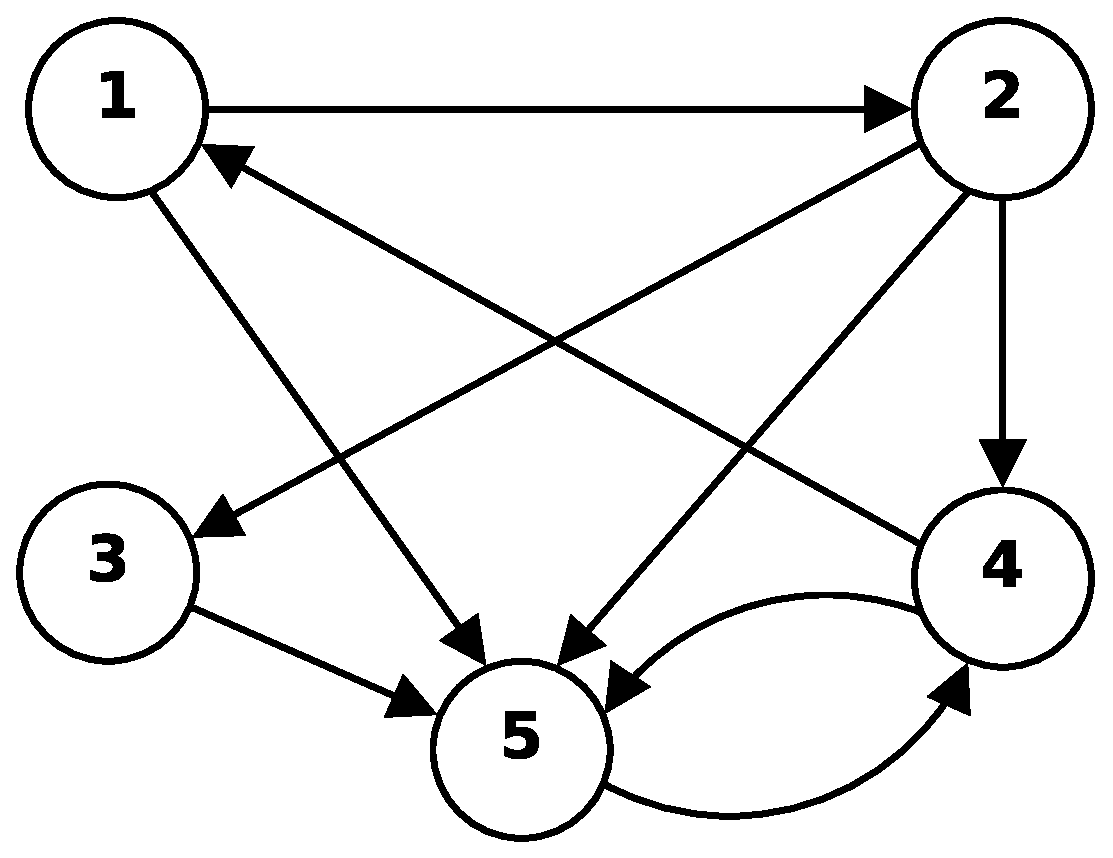
\includegraphics[width=0.5\textwidth]{fig/web}
\caption{Scheme for a 5 pages web. Every circle is a page, every arrow is a
link}
\label{fig:web}
\end{figure}

using the \texttt{Eigen} library, write down a class that computes the maximum
eigenvalue (that is 1) and the corresponding eigenvector, that is the
\emph{pagerank}. Implement also \cpp{operator<<} to see the data inside the
class on the screen.

\subsection*{Soluzione es. 1}

La soluzione dell'esercizio \`e riportata nel seguente listato:
%
\lstset{basicstyle=\scriptsize\sf}
    \lstinputlisting{./es/1/all_in_one/bn-allinone.cpp}
\lstset{basicstyle=\sf}

Si noti, innanzitutto, che \`e stato definito un tipo utente
\cpp{real}. Qualora si volesse modificare la precisione
con cui si effettuano i calcoli, sarebbe sufficiente cambiare solo la
linea contenente la definizione del tipo \cpp{real}. La modifica si
propagherebbe in modo coerente in tutto il codice.

Per rendere l'implementazione dei metodi di ricerca indipendente dalla
funzione considerata si \`e adottata la tecnica dei \emph{puntatori a
funzione}. L'istruzione:
\begin{lstlisting}
typedef real (*fctptr)(real);
\end{lstlisting}
definisce il tipo \cpp{fctptr} come un puntatore a funzioni che
ricevono un argomento di tipo \cpp{real} e restituiscono un valore di
tipo \cpp{real}.

L'arresto dei metodi iterativi per la ricerca degli zeri di una
funzione pu\`o avvenire in base a diversi criteri. Per funzioni che
abbiano derivata prima vicina a $1$ in modulo in corrispondenza dello
zero cercato un efficiente metodo d'arresto \`e basato sul controllo
del \emph{residuo}. In tal caso si considera raggiunta la convergenza
alla prima iterazione $k$ in cui
$\module{\function{f}{x\iter{k}}}<\cpp{tol}$. Un metodo alternativo
basato sul controllo dell'\emph{incremento} risulta, per contro,
efficiente qualora si utilizzino delle iterazioni di punto fisso e la
funzione di iterazione $\function{\phi}{\cdot}$ abbia derivata prima
lontana da $1$ in modulo in corrispondenza dello zero cercato. Tale
criterio prevede l'arresto alla prima iterazione $k$ per cui si abbia
$\module{x\iter{k+1} - x\iter{k}}<\cpp{tol}$. Nel caso del metodo di
Netwon, in cui, per definizione, $\function{\phi'}{\alpha} = 0$, il
controllo dell'incremento fornisce un bilanciamento
ottimale. Nell'implementazione si \`e tenuto conto della
molteplicit\`a dei criteri d'arresto definendo un tipo enumerativo
\cpp{checkT} e dotando ogni metodo di una propriet\`a \cpp{M\_check}
di tipo \cpp{checkT} che specificasse il metodo da utilizzare.

Compilando il codice con i comandi
\begin{verbatim}
    g++ -o bn-allinone bn-allinone.cpp -Wall
\end{verbatim}
Ed eseguendolo, otteniamo
\begin{verbatim}
0.707107        27
0.707107        7
0.707107        14 1
\end{verbatim}


%%%%%%%%%%%%%%%%%%%%%%

\section*{Esercizio 2 - Da svolgere a casa}

In accordo con l'algoritmo per la generazione di mesh non
equi-spaziate descritto in \textit{A. Quarteroni, Modellistica
Numerica per Problemi Differenziali, 4$^a$ edizione} pagina 398,
in basso. Modificare la classe \cpp{Mesh1D} in modo che possa
creare mesh non equi-spaziate partendo da una funzione peso assegnata.

\subsection*{Soluzione es. 2}

Si riporta di seguito il listato dell'\emph{header file} che contiene
le dichiarazioni delle procedure che risolvono l'esercizio.
% zerofun.hpp
\lstset{basicstyle=\scriptsize\sf}
    \lstinputlisting[caption=Procedure per la ricerca
        degli zeri di una funzione.]{es/1/zerofun.hpp}
\lstset{basicstyle=\sf}

Le corrispondenti definizioni sono state inserite nel \emph{source file}
\texttt{zerofun.cpp}:
\lstset{basicstyle=\scriptsize\sf}
    \lstinputlisting[caption=Procedure per la ricerca degli zeri di una
        funzione.]{es/1/zerofun.cpp}
\lstset{basicstyle=\sf}

L'istruzione \texttt{assert(u*f(b)<0.0);} permette un semplice controllo degli errori,
perch\`e provoca l'interruzione del programma e la generazione di un
messaggio di errore se l'espressione \texttt{u*f(b)<0.0} non \`e verificata.

Infine riportiamo il listato contenente il main nel file \texttt{bn.cpp}:
\lstset{basicstyle=\scriptsize\sf}
    \lstinputlisting[caption=Definizione della funzione e main del programma.]
    {es/1/bn.cpp}
\lstset{basicstyle=\sf}

Per la compilazione si ricorre ai seguenti comandi:
\begin{verbatim}
g++  -c -o bn.o bn.cpp -Wall
g++  -c -o zerofun.o zerofun.cpp -Wall
g++  -o bn bn.o zerofun.o
\end{verbatim}

I \emph{files} \texttt{bn.o} e \texttt{zerofun.o} sono la
rappresentazione in codice oggetto delle definizioni di tipi e
funzioni contenute nei \emph{files} sorgente
(rispettivamente \texttt{bn.cpp} e \texttt{zerofun.cpp}.
Il collegamento (\emph{linking}) dei \emph{files} oggetto
produce l'eseguibile \texttt{bn}.
Per disattivare tutti gli \cpp{assert} all'interno del codice,
in fase di compilazione occorre aggiungere il parametro \cpp{-DNDEBUG}
per quei files che utilizzano gli \cpp{assert}, ovvero
\begin{verbatim}
g++  -c -o bn.o bn.cpp -Wall
g++  -c -o zerofun.o zerofun.cpp -Wall -DNDEBUG
g++  -o bn bn.o zerofun.o
\end{verbatim}

Per visualizzare graficamente l'errore commesso, \`e possibile
aggiungere due parametri di input alle funzioni \texttt{bisection},
\texttt{newton} e \texttt{robust}.
Il primo \`e la soluzione esatta mentre il secondo \`e il nome del
file su cui salvare i dati.
Il listato dei comandi contenuti in \texttt{bng.cpp} \`e il seguente:
\lstset{basicstyle=\scriptsize\sf}
    \lstinputlisting[caption=Definizione della funzione e main del programma.]
        {es/1/withGnuplot/bng.cpp}
\lstset{basicstyle=\sf}

Si noti il comando finale di chiamata al sistema operativo,
\`e richiesto quindi il file \texttt{print\_data} che contiene i seguenti comandi
\begin{verbatim}
set terminal png
set output "grafico.png"
plot "data" with lines
\end{verbatim}
I comandi in \texttt{zerofung.hpp} sono sostanzialmente identici a quelli
riportati in \texttt{zerofun.hpp}, mentre i comandi in \texttt{zerofung.cpp}
sono riportati qui di sequito
\lstset{basicstyle=\scriptsize\sf}
    \lstinputlisting[caption=Procedure per la ricerca degli zeri di una
        funzione.]{es/1/withGnuplot/zerofung.cpp}
\lstset{basicstyle=\sf}

Si noti nella funzione \texttt{bisection} e \texttt{newton} la gestione del file.
Anzitutto viene dichiarato, dove \`e necessario l'operatore di scope resolution
\texttt{::} per accedere ai membri definiti nel namespace \texttt{std}.
Successivamente viene aperto in modalit\`a out nel caso della funzione
\texttt{bisection}, mentre in modalit\`a out e app nella funzione \texttt{newton}.
La differenza \`e che nel secondo caso i dati vengono scritti dal fondo del file.
Vi \`e poi un test per verificare se il file \`e stato effettivamente aperto.
All'interno di cicli vi \`e la scrittura dei dati, i comandi sono analoghi a
quelli utilizzati per la visualizzazione a schermo.
Alla fine di entrambe le funzioni il file viene chiuso.

Il grafico ottenuto \`e il seguente
\begin{figure}[!h]
    \centering
    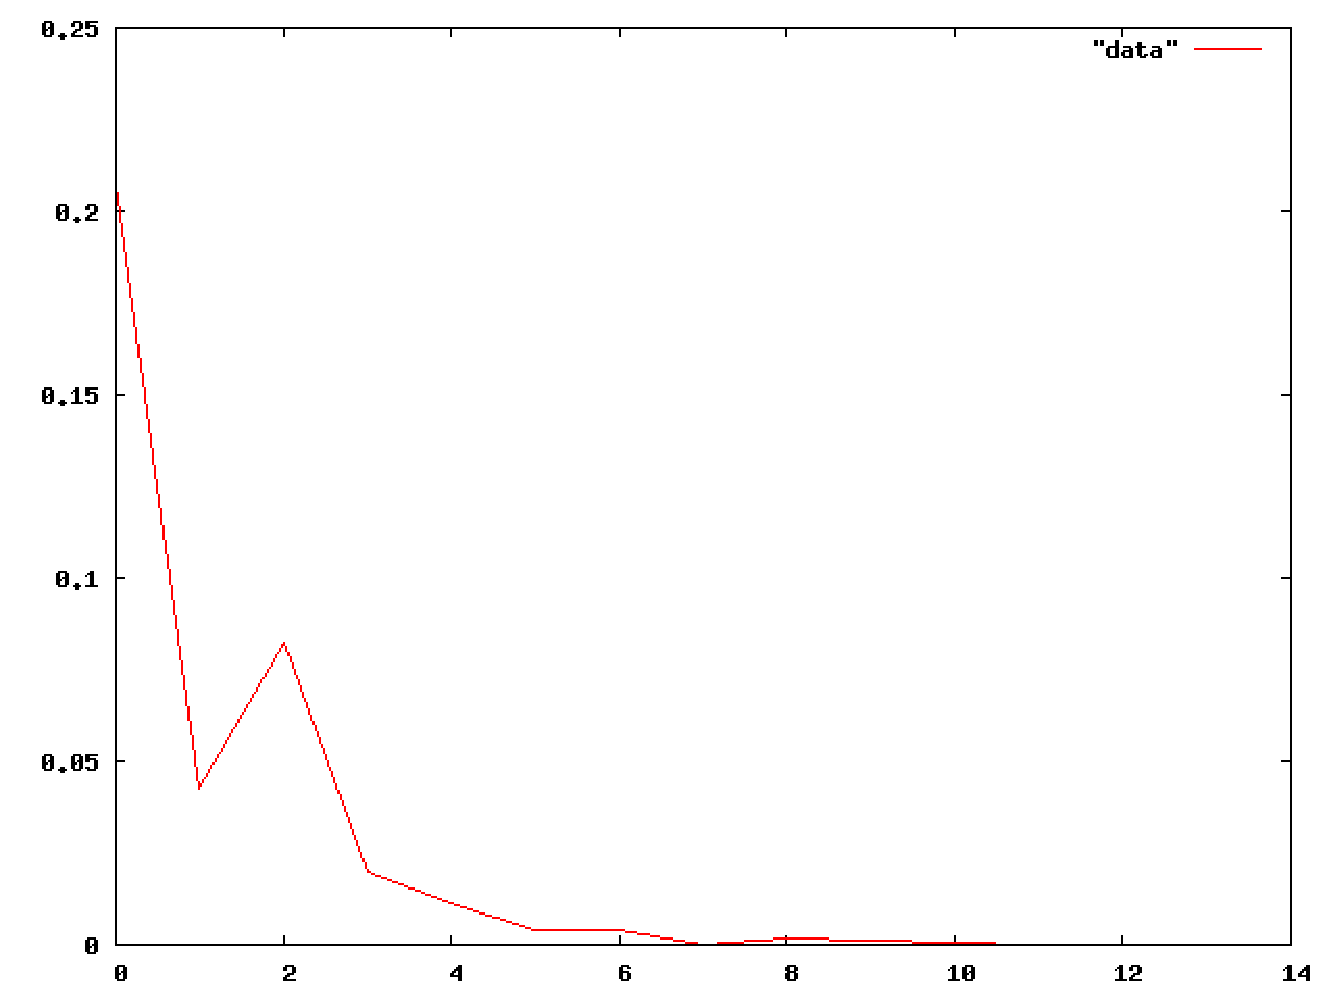
\includegraphics[width=0.7\textwidth]{./images/grafico}
\end{figure}


%%%%%%%%%%%%%%%%%%%%%

\documentclass[12pt,twoside]{article}
\usepackage{amsmath,amssymb}
\usepackage{a4wide}
\begin{document}
Here you find a simple set of codes for the problem: find $\mathbf{x}$ such that
\[
\mathbf{F}(\mathbf{x})=\mathbf{0}
\]
for a $F:\mathbb{R}^n\to\mathbb{R}^n$ (which we assume to be at least Lipschitz continuous).

The set of codes include a class to store non linear systems, a class thet implements Newton method and another for a genetic fixed point iteration.
\section{The class for non linear systems}

\section{The methods implemented}
\subsection{Newton Method}
We indicate with $\boldsymbol{J}(\mathbf{x})$ the Jacobian (Frechet derivative) of $\mathbf{F}$ at $\mathbf{x}$. The algorithm implements a simple backtraching
based on Armijo rule with constant reduction of the step $\lambda$.

Let $\mathbf{x}$ be given, together with a small positive number $\sigma$ and
$\gamma\in (0,1)$
\begin{enumerate}
\item Compute $\mathbf{d}$ by solving
$
\boldsymbol{J}(\mathbf{x})\mathbf{d}=-\mathbf{F}(\mathbf{x}).
$
\item $\lambda=1$.
\item Until $\Vert\mathbf{F}(\mathbf{x}+\lambda\mathbf{d})\Vert< (1-\lambda\sigma)\Vert \mathbf{F}(\mathbf{x}\Vert$ set $\lambda\leftarrow
\gamma\lambda$
\item Set $\mathbf{x}\leftarrow\mathbf{x}+\lambda\mathbf{d}$
\item Check for convergence.
\end{enumerate}
Convergence test is made by checking the residual $\mathbf{F}(\mathbf{x})$, the
step length $\Vert \mathbf{d}\Vert$ and fixing a maximum number of iterations.

Step 3 implements Armijo rule for sufficient decrease of $\Vert\mathbf{F}\Vert$.

\section{Notes}
The architecture of this code can be bettered. First of all one can generalize the class fixed point to accept any iteration function $\boldsymbol{\Phi}(\mathbf{x})$ and implements
\[
\mathbf{x}_{k+1}=\boldsymbol{\Phi}(\mathbf{x}_k), \quad k=1,\ldots
\]
for a given $\mathbf{x}_0$.

In this respect Newton method is just a  particular fixed point iteration with iteration function
\[
\boldsymbol{\Phi}_N(\mathbf{x})=\mathbf{x}-\boldsymbol{J}^{-1}(\mathbf{x})\mathbf{F}(\mathbf{x})
\]

However Newton method can be seen as a particular \emph{line search method}. So one may think to create an abstract class (or a template) for generic line search methods and specialise it for different type of algorithms, using for instance a stategy pattern via policies. Algoritms may include gradient, conjugate gradient (in different forms), Broyden etc etc. It may also implement different backtracking strategies (armijo, Wolfe....) 
All algoritms of the form
\begin{itemize}
\item Compute a descent direction $\mathbf{d_k}$
\item Compute the step $\mathbf{\alpha}_k$ according to a backtracking strategy
\item Update $\mathbf{x}_{k+1}=\mathbf{x}_k+\alpha_k\mathbf{d}_k$.
\end{itemize}
\end{document}
%%% Local Variables:
%%% mode: latex
%%% TeX-master: t
%%% End:


\bibliographystyle{siam}
\bibliography{../common/bibliography}

\end{document}
